\documentclass[12pt]{article}
\usepackage[utf8]{inputenc}
\usepackage[italian]{babel}
\usepackage{amsmath}
\usepackage{mathtools}
\usepackage{stmaryrd}
\usepackage{graphicx}
\title{Verifica automatica della proprietà di\\ sicurezza forte}
\author{Gianluca Lutero}
\date{}

\begin{document}
\maketitle
\thispagestyle{empty}

\newpage
\section*{Introduzione}
In questa relazione verrà descritta una tecnica automatica per la verifica della proprietà di sicurezza forte nei protocolli crittografici. Il metodo in primo luogo formalizza la definizione di segretezza forte come un caso particolare della relazione di equivalenza osservazionale. Definita in questo modo la proprietà viene espresso il protocollo nel formalismo del $\pi$-calcolo esteso con primitive crittografiche. Il protocollo così espresso viene quindi tradotto in un insieme di clausole di Horn le quali ne danno una rappresentazione astratta. Da questa rappresentazione possono essere derivati tutti i test che l'avversario può eseguire per cercare di violare il protocollo. Lo scopo principale quindi è quello di cercare di verificare che nessuno di questi test riveli informazioni segrete senza doverli enumerare tutti, considerando che possono essere infiniti. Questo si ottiene con il nuovo predicato "testunif", il quale non è definito da clausole di Horn ma attraverso specifici passi di semplificazione nell'algoritmo di risoluzione. Considerato questo si può mostrare come il non riuscire a derivare un determinato fatto $bad$, che nel formalismo rappresenta il successo dell'attaccante nel violare il protocollo, il processo preserva la proprietà di segretezza forte.

\newpage
\section*{Calcolo dei processi}
% Descrivere brevemente sintassi e semantica del calcolo dei processi
Per la rappresentazione dei protocolli viene utilizzato il formalismo del calcolo dei processi esteso con le primitive crittografiche probabilistiche. Di seguito viene mostrata la sintassi:\\
\begin{figure}[h]
        \centering
        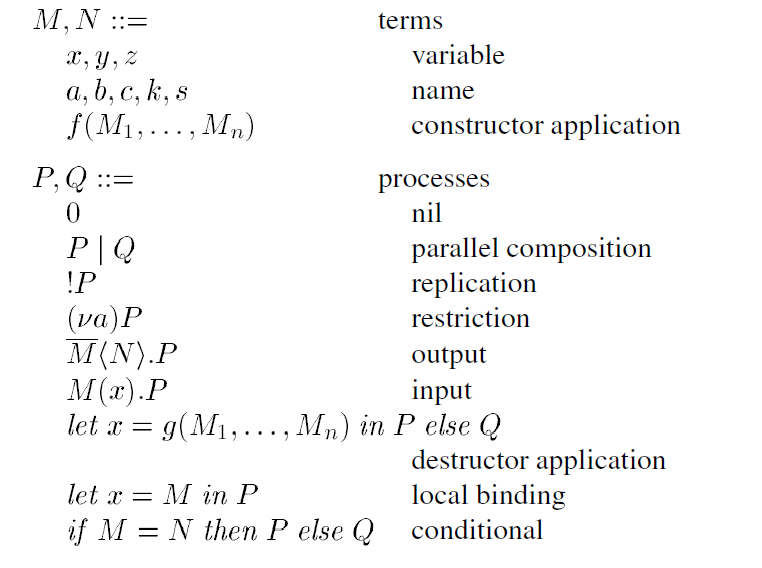
\includegraphics[scale=0.6]{Relazione/Immagini/calcolo.PNG} 
\end{figure}\\
Si assumono un infinito numero di nomi e variabili e un insieme di simboli per i costruttori e i distruttori. Per convenzione vengono usate le lettere $a, b, c, k$ per i nomi, $x, y, z$ per le variabili, $f$ per il costruttore e $g$ per il distruttore. Si definiscono termini le variabili, i nomi e le applicazioni di costruttore. Un distruttore è una funzione parziale che un processo può utilizzare per manipolare termini.\\
L'uso dei costruttori e dei distruttori permette di rappresentare strutture dati e operazioni crittografiche.\\
\begin{center}
 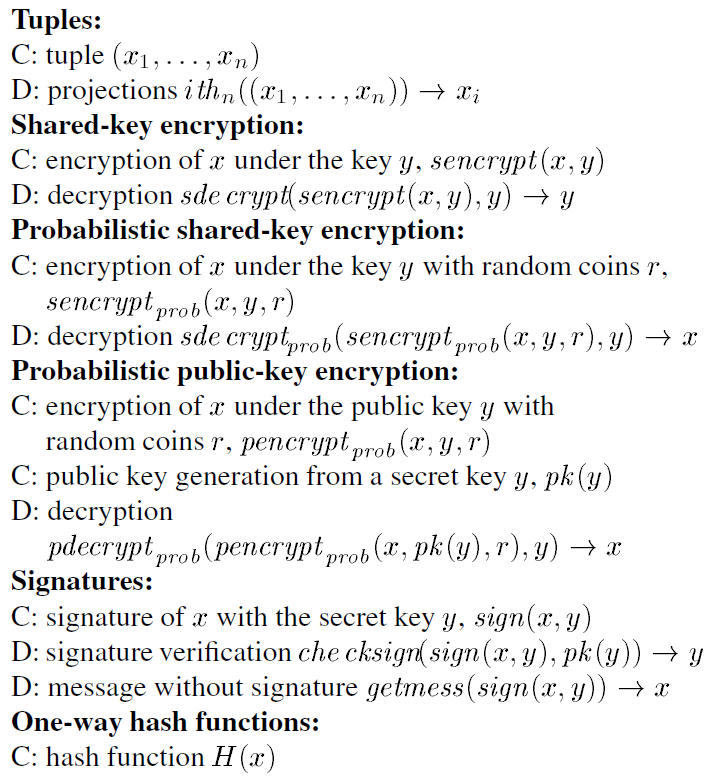
\includegraphics[scale=0.55]{Relazione/Immagini/crypto.PNG}
\end{center}
Vengono definiti inoltre le funzioni $fn(P)$ e $fv(P)$ che restituiscono rispettivamente i nomi e le variabili libere nel processo P. Un processo si dice chiuso se non ha variabili libere. La semantica del formalismo è definita dalla relazione di riduzione $ \xrightarrow{} $ e dalla relazione di equivalenza strutturale $ \equiv$.

\section*{Segretezza forte}
% Definizioni
La proprietà di segretezza forte esprime che un qualsiasi processo che esegue l'attacco non possa rilevare alcuna differenza al variare del valore del segreto. Questa proprietà è più restrittiva rispetto alla tipica nozione di segretezza, che impone all'avversario l'impossibilità di ottenere il valore del segreto, rendendosi necessaria nel momento in cui il valore delle variabili riservate è limitato.
Per formalizzare il concetto si passa dalla definizione di equivalenza osservazionale:\\

\textbf{Definizione:}  Un contesto di valutazione $C$ é un contesto costruito a partire da $[\ ], C | P, P|C \hspace{2mm}e\hspace{2mm} (\nu a)C.$\\
$P$ emette su $m$, $P \Downarrow m$, se e solo se $P (\rightarrow \cup \equiv)^* C[\overline{m}\langle N \rangle.R]$ dove $C$ é un contesto di valutazione che non lega $m$.\\

Si definisce equivalenza osservazionale $\approx$ la piú grande relazione simmetrica $R$ tra processi chiusi tale che $PRQ$ implica:\\
\begin{enumerate}
    \item se $P \Downarrow m$ allora $Q \Downarrow m$
    \item se $P \rightarrow P'$ allora esiste $Q'$ tale che $Q \rightarrow^* Q'$ e $P'RQ'$
    \item $C[P]RC[Q]$ per tutti i contesti di valutazione chiusi $C$.
\end{enumerate}
Un processo $P$ emette su $m$ quando, dopo un qualsiasi numero di passi di riduzione, questi manda un messaggio su $m$ e l'avversario ottiene $m$. In questo modo l'output del canale $m$ é osservabile dall'avversario. Questo fatto é sfruttato nel punto 1 della definizione: per $P$ e $Q$ equivalenti osservazionalmente, se $P$ emette su $m$ allora anche $Q$ emette su $m$, se così non fosse l'avversario sarebbe in grado di distinguerli. Nel punto 2 viene mostrato che la proprietà é preservata dalla riduzione. Questo punto fa sì che la struttura della riduzione sia visibile all'avversario: quando $P$ e $Q$ sono osservazionalmente equivalenti, se $P$ si riduce in modo non deterministico in due processi non equivalenti $P'$ e $P''$, allora anche $Q$ si riduce in due processi $Q'$ e $Q''$ osservazionalmente equivalenti rispettivamente a $P'$ e $P''$. Il punto 3 prende in considerazione l'avversario, rappresentato da un qualsiasi contesto chiuso di valutazione, ossia un contesto di valutazione tale che $C[P]$ e $C[Q]$ sono chiusi. A questo punto può essere data la definizione di segretezza forte attraverso il concetto per cui l'avversario non può distinguere due processi che differiscono per il valore dei messaggi cifrati.\\

\textbf{Definizione:} Il processo $P_0$ preserva la segretezza forte delle sue variabili libere se e solo se per ogni sostituzione chiusa $\sigma$ e $\sigma'$ di dominio $fv(P_0)$ , $\sigma P_0 \approx \sigma' P_0$.\\

Intuitivamente se il processo ha una falla allora esiste un contesto $C$ che può sfruttarla per eseguire differenti output a seconda del valore del messaggio scambiato, per cui $C[\sigma P_0]$ e $C[\sigma' P_0]$ non soddisfano il punto 1 della definizione di equivalenza osservazionale. Viene dato adesso un criterio più forte per dimostrare la segretezza forte. Intuitivamente viene richiesto che per ogni passo di riduzione questa proceda in modo uniforme per tutti i valori dei termini. Per un passo di comunicazione questo significa che il canale deve essere pubblico. Per un distruttore questo significa che il successo o il fallimento del processo sia indipendente dal valore dal messaggio.\\

\textbf{Proposizione 1:} Sia $Secr$ l'insieme dei nomi che contiene tanti elementi quanti sono $fv(P_0)$  e tale che $fn(P_0) \cap Secr = \emptyset$. Sia $\sigma$ una sostituzione che mappa tutte le variabili libere di $P_0$ ad elementi distinti di $Secr$. Si assume allora che per tutti $Q$ tale che $fn(Q) \cap Secr = \emptyset$:
\begin{enumerate}
    \item se $\sigma P_0 | Q (\rightarrow \cup \equiv)^* C[\overline{M} \langle N \rangle . R]$ o $\sigma P_0 | Q (\rightarrow \cup \equiv)^* C[M(x).R]$ e $C$ è un contesto di valutazione tale che non leghi i nomi in $Secr$ allora $M \notin Secr$.
    
    \item se $\sigma P_0 | Q (\rightarrow \cup \equiv)^* C[let\ y\ =\ g(M_0,\dots,M_n)\ in\ Q'\ else\ R']$, $\theta$ è una sostituzione chiusa con $dom(\theta)\ =\ Secr$, $C$ è un contesto di valutazione che non lega nomi di $Secr$ o nelle immagini di $\theta$, $g(N_0,\dots,N_n) \rightarrow N$ è contenuta in $def(g)$, e $\theta (M_0,\dots,M_n)$ è un'istanza di $(N_0,\dots,N_n)$, allora anche $(M_0,\dots,M_n)$ è un'istanza di $(N_0,\dots,N_n)$   
\end{enumerate}
Allora $P_0$ preserva la proprietà di segretezza forte.\\

Il processo $Q$ rappresenta un qualsiasi avversario. Il secondo punto della proposizione indica che se l'applicazione di un distruttore $g(M_0,\dots,M_n)$ ha successo per il valore dei messaggi dati da $\theta$ allora deve avere successo per qualsiasi valore del messaggio.\\ 

\textbf{Dimostrazione:} Per procedere devono prima essere riformulate le proposizioni precedenti usando il concetto di contesto per rappresentare l'avversario. Sia $C$ un contesto di valutazione. Sia $Secr'$ un insieme di nomi non libero o legati in $C$ e non liberi in $P_0$, contenenti tanti elementi quanti $fv(P_0)$. Sia $\sigma'_0$ una sostituzione che mappa le variabili libere di $P_0$ in $Secr'$.
\begin{enumerate}
    \item se $C[\sigma'_0 P_0] (\rightarrow \cup \equiv)^* C'[\overline{M} \langle N \rangle . R]$ o $C[\sigma'_0 P_0] (\rightarrow \cup \equiv)^* C'[M(x).R]$ e $C'$ è un contesto di valutazione che non lega nomi in $Secr'$ allora $M \notin Secr'$.
    \item se $C[\sigma'_0 P_0] (\rightarrow \cup \equiv)^* C'[let\ y\ =\ g(M_0,\dots,M_n)\ in\ Q'\ else\ R']$, $\theta$ è una sostituzione chiusa con $dom(\theta)\ =\ Secr'$, $C'$ è un contesto di valutazione che non lega nomi di $Secr'$ o nelle immagini di $\theta$, $g(N_0,\dots,N_n) \rightarrow N$ è contenuta in $def(g)$, e $\theta (M_0,\dots,M_n)$ è un'istanza di $(N_0,\dots,N_n)$, allora anche $(M_0,\dots,M_n)$ è un'istanza di $(N_0,\dots,N_n)$ 
\end{enumerate}
Si definisce ora la relazione $R$ come $PRP'$ se e solo se esiste:\\
\begin{enumerate}
    \item un contesto di valutazione $C$
    \item un insieme $Secr'$ di nomi non liberi o legati in $C$ e non legati in $P_0$, contenenti tanti elementi quanti sono in $fv(P_0)$
    \item una sostituzione $\sigma'_0$ che mappa le variabili libere di $P_0$ ad elementi distinti di $Secr'$
    \item sostituzioni $\theta$ e $\theta'$ con dominio $Secr'$
    \item un processo chiuso $P''$ tale che $P\ =\ \theta P''$, $P'\ =\ \theta'P''$ e\\ $C[\sigma'_0 P_0]\ (\rightarrow \cup \equiv)^*\ P''$  
\end{enumerate}
La relazione $R$ è simmetrica. Si dimostra adesso che $R$ soddisfa i tre punti della definizione di equivalenza osservazionale.\\
\begin{itemize}
    \item La prova del punto 1 avviene usando l'ipotesi 1 mostrando che il canale non viene modificato da $\theta$ e $\theta'$
    \item La prova del punto 2 viene fatta per casi sulle riduzioni. Nel caso di una comunicazione viene usata l'ipotesi 1 per mostrare che il canale non viene modificato da $\theta$ e $\theta'$, in questo modo $ P\ =\ \theta P'',\ P'\ =\ \theta'P'' $ e $P''$ possono comunicare.Il caso dell'applicazione del distruttore usa l'ipotesi 2: se l'applicazione del distruttore ha successo in $P\ =\ \theta P''$ allora ha successo anche per $P''$ e $P'\ =\ \theta'P''$; se il distruttore fallisce in $P$ allora fallisce sia in $P''$ e $P'$ dato che se avesse avuto successo in $P'\ =\ \theta'P''$ per l'ipotesi 2 avrebbe implicato il successo anche in $P''$ e $P\ =\ \theta P''$
    \item La prova del punto 3 si basa sulla definizione di $R$. Il punto delicato della dimostrazione risiede nel rinominare i nomi in $Secr'$ per impedire la loro cattura dal contesto aggiunto
\end{itemize}
Allora $R \subset \ \approx$. In più per ogni sostituzione $\sigma$ e $\sigma'$ di dominio $fv(P_0)$ vale $\sigma P_0 R \sigma'P_0$, prendendo $C=[\ ],\ Secr'\ =\ Secr,\ \sigma'\ =\ \sigma, \theta \ e\ \theta'$ tali che $\theta \sigma_0 \ =\ \sigma,\ e\ \theta'\sigma_0\ =\ \sigma', P'\ =\ \sigma_0 P_0$. In questo modo $P_0$ preserva la proprietà di segretezza forte delle sue variabili libere.

\section*{Primitive per la verifica del protocollo}
Adesso verrà esteso il formalismo per la verifica dei protocolli con le primitive per la verifica della proprietà di segretezza forte. Il sistema di verifica costruisce un insieme di clausole di Horn a partire da un processo chiuso $P_0$. Si assume che ogni restrizione $(\nu a)P$ in $P_0$ contiene un nome differente per $a$ e che quel nome sia differente per ogni nome libero in $P_0$. Si associa ad ogni replicazione in $P_0$ un identificare di sessione. Gli identificatori di sessione sono variabili che prendono valore da un insieme numerabile di termini e un valore diverso per ogni copia del processo replicato. Questo permette di distinguere le diverso copie del processo, in particolare vengono usati per distinguere i nomi generati dalle stesse restrizioni nelle differenti copie del processo. I termini delle regole sono chiamati pattern $p$ e sono generati dalla seguente grammatica:\\
\begin{figure}[ht]
    \centering
    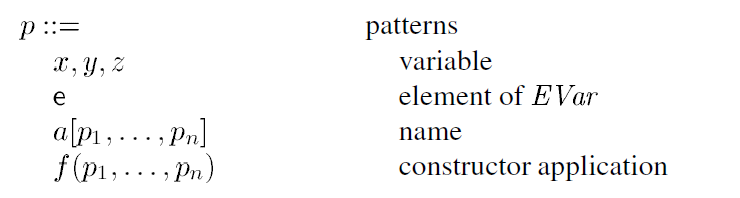
\includegraphics[scale=0.7]{Relazione/Immagini/rule.PNG}
\end{figure}\\
L'insieme $EVar$ contiene le costanti usate nel predicato $testunif$. Una restrizione in un processo crea sempre un nuovo nome ogni volta che questi viene eseguito. Quando una restrizione si trova all'interno di una replicazione, questo porta a generare un illimitato numero di nomi, il che porta alla non terminazione della procedura se questi vengo rappresentati in modo diretto. Per evitare questo i nomi vengono rappresentati come funzioni. Le regole si basano sui seguenti fatti:\\   
\begin{figure}[h]
    \centering
    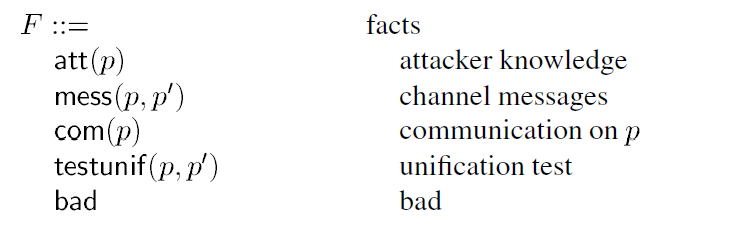
\includegraphics[scale=0.6]{Relazione/Immagini/fatti.PNG}
\end{figure}\\
Il fatto $att(p)$ significa che l'avversario può conoscere il valore di $p$. Il fatto $mess(p,p')$ sta a significare che il messaggio $p'$ può comparire sul canale $p$. Il fatto $com(p)$ sta a significare che l'avversario può comunicare sul canale $p$, il che permette ad esso di verificare che $p$ sia un nome oppure no. Il predicato $bad$ serve per rilevare il caso in cui viene violata la proprietà di segretezza forte. Il fatto $testunif(p,p')$ è definito come segue. Si dice che un insieme di pattern contengono nomi legati quando contengono sottotermini della forma $a[\dots]$ dove $a$ corrisponde ad una restrizione nel processo. Nella seguente definizione si utilizzano $Secr$ e $\sigma_0$ come nella Proposizione 1.\\
\\
\textbf{Definizione 3:} Siano $p,p'$ pattern chiusi. Si dice che $testunif(p,p')$ è vero se e solo se esiste una sostituzione chiusa $\sigma$ di dominio $Secr\ \cup \ EVar $ tale che $\sigma Secr$ non contiene nomi legati e $\sigma p = \sigma p'$, e non esiste una sostituzione $\sigma'$ di dominio $EVar$ tale che $\sigma' p = \sigma' p'$.\\
\\
Quello che si intende nella definizione è che il predicato $testunif(p,p')$ restituisce vero quando l'esito del processo di unificazione di $p$ e $p'$ dipende dal valore del messaggio.\\
Adesso verranno descritte le regole che rappresentano le abilità dell'avversario e le azioni degli altri partecipanti.\\
\\
\textbf{Regole per l'avversario } Di seguito verranno riportate le regole che rappresentano le azioni che un qualsiasi processo $Q$, che rappresenta l'avversario, possa fare.\\

\begin{figure}[ht]
    \centering
    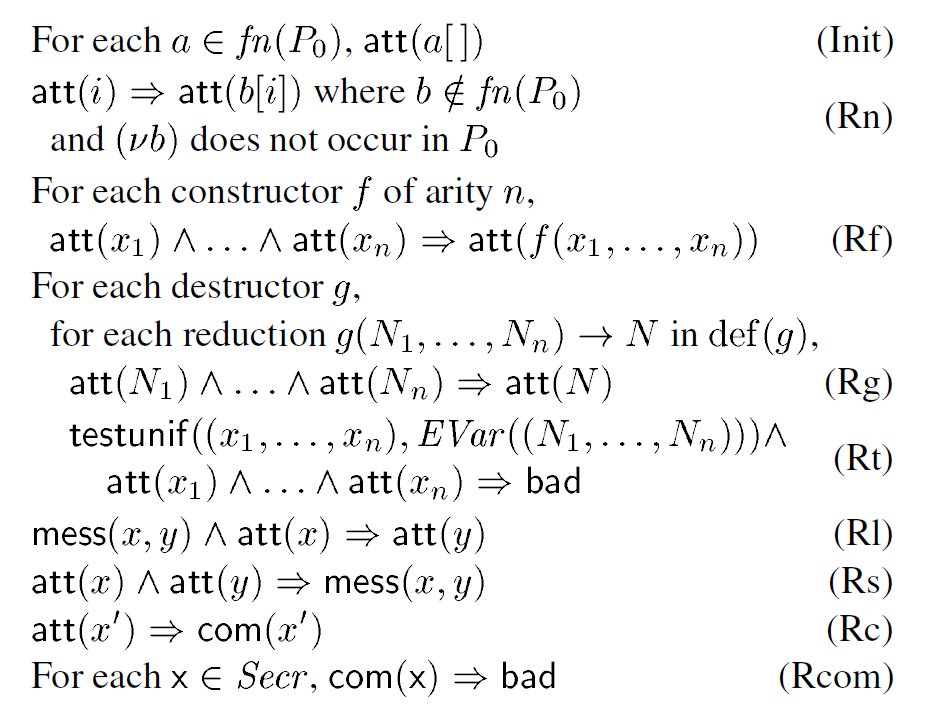
\includegraphics[scale=0.4]{Relazione/Immagini/term_rule.PNG}
\end{figure}
La regola $(Rc)$ sta a significare che se l'avversario ha $x'$ allora può iniziare una comunicazione su di esso. La regola $(Rcom)$ controlla che $com(x)$ non sia derivabile da $x \in Secr$, in questo modo non avviene alcuna comunicazione sui canali di  $Secr$. Quando tutte le comunicazioni avvengono su un canale pubblico costante questo equivale a mostrare che $att(x)$ non è derivabile, questo è il criterio per dimostrare la proprietà di segretezza standard di $x$. La regola $(Rt)$ sta ad indicare che se l'avversario ha $x_0,\dots,x_n$ allora può verificare se il distruttore ha avuto successo oppure no. Quindi se $testunif((x_0,\dots,x_n),EVar((M_0,\dots,M_n)))$ è vero indica che se per qualche valore del segreto $(x_0,\dots,x_n)$ è un'istanza di $(M_0,\dots,M_n)$ ma non per altri, allora potrebbe esserci un attacco per violare la segretezza forte. La regola $(Rn)$ descrive il fatto che un avversario può generare un numero illimitato di nuovi nomi $b[i]$. La regola $(Init)$ indica che l'avversario inizialmente conosce tutti i nomi liberi di $P_0$. Le regole $(Rf)$ e $(Rg)$ stanno ad indicare che l'avversario può applicare tutte le operazione ai termini che conosce. La regola $(Rl)$ indica che l'avversario può ascoltare da ogni canale che conosce mentre con la regola $(Rs)$ può mandare messaggi a tutti i canali che conosce.\\

\textbf{Regole per il protocollo } La traduzione di $\llbracket P \rrbracket \rho sh$ di un processo $P$ è un insieme di regole dove $\rho$ è una funzione che associa un pattern ad ogni nome e variabile, $s$ è una sequenza di pattern e $h$ una sequenza di fatti. La sequenza vuota è indicata con $\emptyset$, la concatenazione di pattern come $s,p$ e la concatenazione di fatti come $h \land F$.\\
\begin{center}
    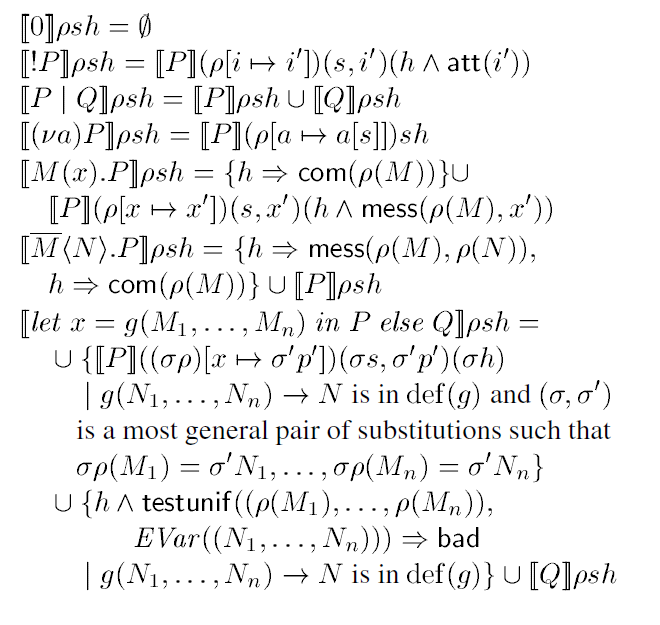
\includegraphics[scale=0.7]{Relazione/Immagini/semantic.PNG}
\end{center}
L'ambiente $\rho$ mappa nomi e variabili al loro corrispondente pattern. La sequenza $s$ contiene tutti i messaggi di input, gli identificatori di sessione e i risultati dei distruttori fino a quel punto del programma. La sequenza $h$ contiene tutti i fatti che devono essere veri fino al punto corrente del programma. 
\section*{Algoritmo di risoluzione}
L'algoritmo inferisce nuove proposizioni per risoluzione come segue. A partire da due proposizioni $R\ =\ H \Rightarrow C$ e $R'\ =\ F \land H' \Rightarrow C'$ si ottiene che $R \circ_F R'\ =\ \sigma H \land \sigma H' \Rightarrow \sigma C'$ dove $C$ e $F$ sono unificabili e $\sigma$ è il più generico unificatore per $C$ e $F$:\\
\begin{center}
    \Large
    $\frac{H\Rightarrow C \hspace{2cm} F \land H' \Rightarrow C'}{\sigma H \land \sigma H' \Rightarrow \sigma C'}$
\end{center}
La proposizione $R \circ_F R'$ è la combinazione di $R$ e $R'$, in cui $R$ prova le ipotesi $F$ di $R'$. La risoluzione è guidata dalla funzione di selezione $sel$: $sel(R)$ ritorna un sottoinsieme delle ipotesi di $R$ e il passo di risoluzione successiva viene effettuata solo quando $sel(R)\ =\ \emptyset$ e $F \in sel(R')$. In questo caso viene usata la seguente funzione di selezione:\\
\begin{itemize}
    \item quando la proposizione è \\$R = testunif((x_1),(x_2))\ \land \ att(x_1)\ \land \ att(x_2)\ \Rightarrow \ bad$:\\
    
    $sel(R) = \{att(x_1)\}$
    \item per tutte le altre proposizioni $sel(R)$ è definita come:\\
    
    $
    sel(H\ \Rightarrow \ C)\ =\  
    \begin{cases} 
    \emptyset & \text{se tutti gli elementi di H sono nella forma } \\
    &  att(x) \text{, con x variabile, o testunif(p,p')} \\
    \{F\} & \text{dove } F\ \neq \ att(x), F\ \neq \ testunif(p,p'),\\
    & \text{con } F \in H, \text{ altrimenti}
    \end{cases}
   $
 \end{itemize}
 
 Nell'ultimo caso possono esserci più scelte per $F$, per semplicità se ne sceglie una casualmente. La funzione di selezione non deve mai scegliere il fatto $testunif$ perchè non è definito da proposizioni. Non dovrebbe essere scelto neanche $att(x)$ perchè questo porterebbe a non terminazione. Però se $att(x)$ non venisse selezionata nel primo caso della funzione di selezione questa rimarrebbe invariata dopo l'applicazione dell'algoritmo portando a non sapere se il fatto $bad$ possa essere derivabile oppure no da questa regola. L'algoritmo usa ottimizzazioni standard, come l'eliminazione delle tautologie eseguita dalla regola $eliminataut$, e anche specifiche per i protocolli, come l'eliminazione dell'ipotesi $att(x)$: $elimattx$ rimuove l'ipotesi $att(x)$ quando $x$ non appare da altre parti nella proposizione, questo può essere fatto in quanto l'ipotesi risulta essere sempre vera finché l'attaccante risulta avere almeno un termine. Per determinare se $testunif(p_1,p_2)$ è vero oppure no bisogna estendere l'algoritmo. Questo si ottiene attraverso una tecnica specifica di semplificazione. Le semplificazioni hanno diversi obiettivi: ridurre le dimensioni dei fatti $testunif$, in modo tale che questi non crescano in modo indefinito; progredire verso la conoscenza del valore di verità di questi fatti instanziando le variabili; semplificarli quando il loro valore di verità è noto. Le semplificazioni che possono essere raggruppate in una funzione $simplify$ definita come segue :\\
 \begin{center}
     $simplify\ =\ elimtaut\ \circ \ elimattx\ \circ \ simptestuniftrue\ \circ \ simptestuniffalse\ \circ \ repeat(elimvar\ \circ \ instantiate\ \circ \ elimEVar\ \circ \ swap\ \circ \ unify) $
 \end{center}
 
 L'espressione $repeat(f)$ sta a significare che la funzione $f$ viene ripetuta finchè non viene raggiunto un punto fisso. È sufficiente ripetere la semplificazione solo quando $elimvar$ o $instantiate$ hanno modificato l'insieme delle proposizioni. La ripetizione non porta a loop infinito perchè le dimensioni di $testunif$ decrescono ad ogni iterazione. Viene definita la funzione $condense(R)$ che applica $simplify$ ad $R$ ed elimina da essa le proposizioni sussunte. Si dice che $H_1\ \Rightarrow \ C_1$ sussume $H_2\ \Rightarrow \ C_2$ se e solo se esiste una sostituzione $\sigma$ tale che $\sigma C_1 \ =\ C_2$ e $H_1 \subseteq \ H_2$. Se \textit{R} contiene le proposizioni $R$ e $R'$, tali che $R$ sussume $R'$, allora la proposizione $R'$ viene eliminata. Si definisce ora l'algoritmo $saturate(R_0)$. Iniziando da $condense(R_0)$, l'algoritmo aggiunge le proposizioni inferite dalla risoluzione con funzione di selezione $sel$ e condensa l'insieme delle proposizioni ad ogni passo di iterazione finchè non viene raggiunto un punto fisso. Quando viene raggiunto il punto fisso, $saturate(R)$ è l'insieme delle proposizioni $R$ nell'insieme delle proposizioni ottenute tale che $sel(R)\ =\ \emptyset$. Il seguente lemma mostra come alla terminazione dell'algoritmo l'unica proposizione rimanente che contiene $bad$ è $bad$ stesso. Quindi $bad$ è derivabile da $saturate(R_{P_0})$ se e solo se la proposizione $bad$  è contenuta in $saturate(R_{P_0})$. \\
 
 \textbf{Lemma}: Dopo la semplificazione, se $R\ =\ H \Rightarrow \ bad$ e $H$ è non vuoto, allora $sel(R)\ \neq \ \emptyset$.\\
 
 L'algoritmo sopra descritto genera la proposizione $bad$ se e solo se $bad$ è derivabile da $R_{P_0}$. Quindi se non può essere generata la proposizione $bad$ allora $P_0$ preserva la segretezza forte delle sue variabili libere.
 
 \newpage
 \begin{thebibliography}{}
    \bibitem{strong_secrecy}
    B. Blanchet, "Automatic proof of strong secrecy for security protocols," IEEE Symposium on Security and Privacy, 2004. Proceedings. 2004, Berkeley, CA, USA, 2004, pp. 86-100.
    \bibitem{tutorial}
    Bruno Blanchet, Ben Smyth, Vincent Cheval, and Marc Sylvestre, "ProVerif 2.00:Automatic Cryptographic Protocol Verifier, User Manual and Tutorial", 2018 
    \bibitem{textbook}Jonathan Katz,Yehuda Lindell,"Introduction to Modern Cryptography"
 \end{thebibliography}
 \end{document}